\chapter{Background}

\section{Medical Imaging}
The field of medical imaging came into existence with the discovery of x-rays in 1895 by Wilhelm R\"{o}ntgen\cite{rontgen}. This meant that for the first time it was possible to peek into the human anatomy without having to physically open it up. This revolution came at a cost however as at the time the dangers of high doses of radiation were not understood and many of the pioneers died as a result of exposure\cite{xraydeath}.

Radiology, the use of ionizing radiation to image objects, was greatly refined over the years; contrast agents were developed which made fields like angiography (imaging of blood vessels) possible\cite{infinityhistory} and the doses used were refined to dramatically decrease the associated risks. X-rays have been used successfully in medical imaging ever since and in the 70s the invention of the CT scanner allowed them to be used to produce 3D images of the body.

It was not until the 1980s that magnetic resonance imaging (MRI) was first used for medical diagnosis. MRI is based on the principles of nuclear magnetic resonance (NMR), which had been used in chemical analysis since the 40s\cite{bshr:mallard}.

MRI can be used to create anatomical images by examining the varying water content in different parts of the body. More recently MRI has been used to create functional images of the brain by using the same principals to detect blood flow\cite{fmri}. Unlike CT, which uses x-rays, MRI does not require the use of any ionizing radiation to perform the scan.

As with all medical imaging techniques the benefits and risks need to be weighed up before a scan is performed. When imaging fetuses the risks are higher than normal and so in general CT scans tend not to be used wherever possible. MRI however, like US (ultrasound), is not associated with known adverse fetal effects.\cite{pregnancyimagingguidelines}

\subsection{MRI (Magnetic Resonance Imaging)\cite{howmriworks}}

MRI is a medical imaging technique that uses a strong magnetic field and radio waves to produce images of the body. MRI can be used to produce 2D, 3D and even 4D images and has the advantage that it doesn’t use any ionizing radiation during the scanning process.

MRI is able to detect the amount of water that is contained in different types of tissue in the body by exploiting a property of protons called spin. Each water molecule in the body contains two hydrogen atoms and the nucleus of each is simply a proton.

MRI applies a strong uniform magnetic field to the area being imaged which causes the spins of the protons to line up with the direction of the field. Some of the protons line up in the same direction, with low energy, and some line up opposing the magnetic field, which have high energy.

When a radio wave is then applied some of the lower energy protons flip to become higher energy and oppose the magnetic field, when the radio waves are stopped these protons then flip back and emit a radio wave that can be detected.

The resonant frequency of radio wave that is required to excite the protons depends on the strength of the magnetic field. This property allows an area to be scanned by applying a gradient magnetic field and varying the radio frequency.

There are a number of different variations of MRI. T1-weighted scans are best for visualising fat, calcification, hemorrhage, thyroid, liver and bone marrow whereas T2-weighted scans accentuate water content.
There are also a number of different ways of acquiring the scan. SSFSE (Single Shot Fast Spin Echo) works by acquiring each slice of the image in sequence whereas 2DGRE (Gradient Echo) acquires all of the slices simultaneously.

If the contrast that can be achieved with MRI is insufficient for the imaging then a contrast agent, such as gadolinium, can be administered to enhance the quality of the image.

\subsection{Fetal MRI\cite{fetalmri}}

Since MRI, like US, is a non-invasive procedure that doesn’t use ionizing radiation it is ideal for use in fetal imaging. While US remains the most common imaging modality used during pregnancy MRI has a number of advantages; in particular it has better contrast in soft tissue which allows individual organs to be better differentiated. US however remains the cheaper of the two and is unlikely to be replaced as the main fetal imaging tool in the near future.

There are no known side effects associated with using MRI, however it is currently recommended to wait until the 17th or 18th WG (week of gestation) before performing MRI. This is partly a precautionary measure but also before then the size of the fetus and amount of movement limits the usefulness of the scan.

\newpage
\subsection{Super Resolution\cite{superresolution1}\cite{superresolution2}}
One of the challenges with using MRI for fetal imaging the resolution that is achievable with current scanners. A typical slice thickness when performing a scan on a fetal brain for example is 3mm, which is set to provide a good balance between resolution and noise. Comparing this to the brain, which may only be 5cm, limits the diagnostic potential.

Super resolution is a technique that is designed to address this issue. The idea behind super resolution is to construct a higher resolution image by combining information from multiple lower resolution images. A similar approach is used in stereoscopic 3D where the information from two images taken from different perspectives are combined to create one 3D image.

In the case of super resolution two (or more) images are taken such that the translation between them known to subpixel accuracy. Having images where the pixels are interleaved in this way allows a higher resolution image to be constructed by interpolation of these images.

\begin{figure}[h]
    \centering
	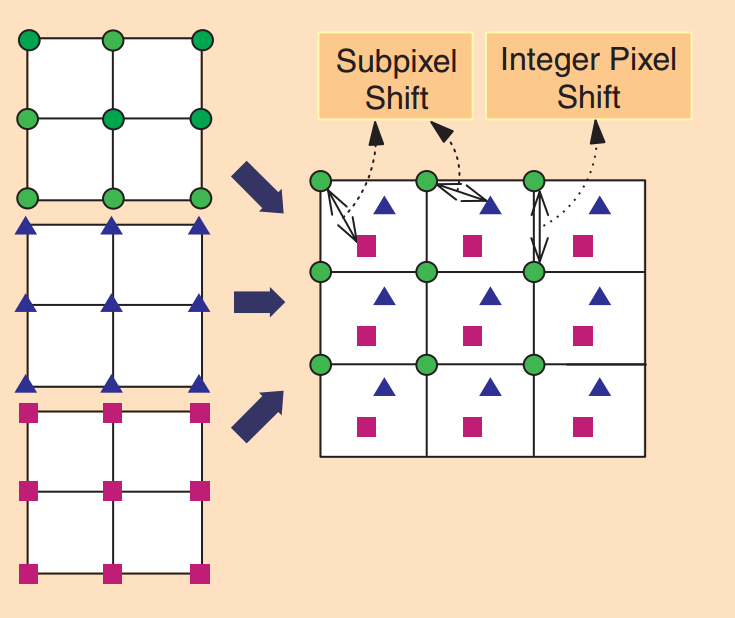
\includegraphics[width=0.8\textwidth]{images/super_resolution.png}
    \caption{Many low resolution images are aligned to sub-pixel accuracy. Adapted from \cite{superresolution2}}
    \label{fig:superresolution}
\end{figure}

\subsubsection*{Intuitive Super Resolution Overview}
The most simple form of super resolution follows three steps:

\begin{enumerate}
	\item Registration
	\item Interpolation
	\item Post-processing
\end{enumerate}

The registration step is where the translation between each image is established. Crucially this must be known to subpixel accuracy and must not be an integer number of pixels. If, for example, we had two images and one was taken exactly 1 pixels width to the right of the other then we see that both images will contain the same amount of information, in effect we can generate one using the other. However, if the second image is known to be taken half a pixels width to the right then there is the potential to extract more information.

Once we have registered our images we then interpolate points at a higher resolution, using a combination of the pixel values from each image at each point. There are a number of different interpolation algorithms that we can use; for example nearest neighbour or (bi)linear interpolation.

We can then take our final outputted image and apply some post-processing effects to reduce the noise or blur. For example, we could apply a Wiener filter\cite{wienerfilter}.

\subsubsection*{Details}
To understand the uncertainty that is introduced we must look more closely at how it works.
To begin with we model the process that happens when a discrete, low resolution image is taken of a continuous scene in the real world. We can express the low resolution images in terms of a perfect, non-aliased, high resolution version which, in an ideal world, we would like to recover. From the Shannon-Nyquist sampling theory an accurate representation is one that is sampled at twice the frequency of the real world signal\cite{shannonnyquist}. In our model we will assume that the resolution of our perfect image is $LN * LN$, our actual camera takes images at the resolution of $N * N$ and the scale factor between the two is $L$.

There are a number of effects that combine to create the final image during acquisition. Each image may be taken from a different position so we will need to account for translations, rotations or other warping. Then various optical effects, such as the limit of diffraction, aberrations or being out of focus, will cause some degree of blurring. Finally the image will be sampled at the resolution of the camera and a certain amount of noise will be present.

These processes can be represented by a series of transformations that can be applied to our ideal image.

\begin{align*} 
& y = DBMx + n \nonumber \\ 
& \text{where} \\
& y \text{ - low resolution image} \nonumber \\
& x \text{ - high resolution (ideal) image} \nonumber \\
& M \text{ - warping (translation, rotation)} \nonumber \\
& B \text{ - blurring (optical effects, motion blur)} \nonumber \\
& D \text{ - scaling (discrete sampling)} \nonumber \\
& n \text{ - noise} \nonumber
\end{align*}

The task of image super resolution is given a number of these such images $y$, can we reverse the process to find $x$, our high resolution version.

Finding $M$ is a case of estimating the movement between each of the images that we have. Depending on the application finding these translations can be a very difficult task; in the case of MRI we are dealing with a controlled environment and so it is possible to take images with a known relationship to each other. If the target remains stationary, this makes finding the translations straight-forward, however dealing with movement (such as breathing) makes this a significantly harder task.

Finding B requires modelling the optical effects that occur at each pixel. This will vary between devices and is normally modelled by a point spread function (PSF) that is a spatial averaging of the pixel values in the area. The PSF can be assumed to be the same throughout the image, known as linear space invariant (LSI), or can vary across the image, known as linear space variant (LSV). An example where a linear space variant PSF would be suitable is where there is more heavy blurring near the edge of an image.

The matrix $D$ then samples the result to produce a lower resolution, aliased image and then some noise, $n$, is added to model random variation in the sensor.

These matrices can be combined to give us this result, without loss of generality:

\begin{align}
& y = Wx + n \nonumber
\end{align}

There are a number of different processes that are used to try and reverse this process. In particular we can see that we will have different confidence in each pixel based on:

\begin{enumerate}
	\item sampling - If we sample our new image too finely then a lot of the pixels will just blend together yielding no new information.
	\item registration - Depending on the calibration of the scanner we will know the registration values to within a certain tolerance.
	\item bias/intensity.
\end{enumerate}

% TODO: Work out what bias is.

\newpage
\subsection{Singular Value Decomposition and Principal Component Analysis}
SVD breaks down a matrix, $A$, into three components: $U$, $D$ and $V$.

\begin{align}
& A = UDV* \nonumber \\
& \text{where} \nonumber \\
& A \text{ - the original matrix, M x N.} \nonumber \\
& U \text{ - a unitary matrix, M x M.} \nonumber \\
& D \text{ - a diagonal matrix containing the singular values, M x N.} \nonumber \\
& V* \text{ - the conjugate transpose of V, a unitary matrix, N x N.} \nonumber
\end{align}

NOTE: Unitary Matrix means that $UU* = I$ or alternately $U^{-1} = UT$. This is true where the matrix contains unit vectors.

NOTE: The conjugate transpose ($*$) of a matrix is where you take the transpose and then take the complex conjugate of each cell.

SVD on it’s own isn’t particularly exciting, but it comes in handy when doing PCA. PCA is used to take a dataset in n dimensions and map it in a way that allows you to describe it in fewer, whilst minimizing the information lost.

PCA takes in a data matrix, this is just a two dimensional table where each row represents an experiment or data point and each column is a particular property. PCA works off the covariance of this data, to see how each property varies with relation to each other property.

To find the principal component we would like find the vector that maximizes the variance in the covariance matrix. This can be found by extracting the eigenvalues of the covariance matrix.

\begin{align*}
& X \text{ - data matrix (demeaned)} \\
& XX^{T} \text{ - covariance matrix} \\
& \\
& \text{Since the covariance matrix is symmetric it can be diagonalized.} \\
& \\
& XX^{T} = WDW^{-1} \\
& \\
& W \text{ - eigenvectors of the covariance matrix} \\
& D \text{ - eigenvalues of the covariance matrix} \\
\end{align*}

We can use PCA on $X$:

\begin{align*}
X &= UDVT \\
& \\
XXT &= (UDVT)(UDVT)T \\
	&= (UDVT)(VDTUT) \\
	&= UDDTV \\
	&= UD^{2}U \\
	& \text{therefore} \\
UD^{2}U &= WDW
\end{align*}

We see that the eigenvalues are just the square root of the diagonal we get from SVD and the eigenvectors are the same.

Principal component analysis, or a slightly modified version of it, may be applicable when suggesting the next scan plane based on the uncertainty information.

\newpage
\subsection{RANSAC}
RANSAC, which stands for Random Sample Consensus, is a technique for estimating model parameters given some sample data.

Consider the task of trying to fit a line to some data which contains both correct points (inliers) and noisy data (outliers). The problem with simply minimizing the sum of squared errors to all of the points is that the outliers will distort the result such that the inliers are not perfectly described by the data. Figure~\ref{fig:ransac} illustrates this task.

\begin{figure}[h]
    \centering
	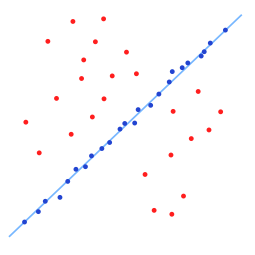
\includegraphics[width=0.4\textwidth]{images/ransac.png}
    \caption{Inliers are shown in blue, outliers shown in red. From \cite{ransac:image}}
    \label{fig:ransac}
\end{figure}

RANSAC gets over this problem using random sampling and iteration. It relies on there being more inliers than there are outliers so that statistically inliers will be chosen more frequently. The algorithm is composed of two steps which are repeatedly applied.

As many points are taken randomly from the data set as are needed to fully specify the model. e.g. you need two points to specify a line.

The model is fit to these points. e.g. by minimizing the sum of squared differences.
All of the data points are compared to this model. If they differ by more than a threshold value they are discarded. If they fit the model they are put into this iterations ‘inlier set’.

A number of iterations are then performed and the winning iteration is the one with the largest inlier set. The final model is then either the model which gave the largest inlier set or alternatively the model can be generated using every point in the inlier set.
This algorithm relies on certain parameters being tweaked to perform well.

\begin{itemize}
	\item threshold (how picky to be when discarding points)
	\item iterations (how many times to perform the algorithm)
\end{itemize}

RANSAC may be of use in this project to pick the next scan plane given our uncertainty values. The scan plane will be chosen such that it provides the most information, given the uncertainty, and so in this case you can imagine using it to fit a ‘plane’ to the uncertainty values.

The algorithm will need to be modified to account for the three types of uncertainty that the visualisation uses and some experimentation will be needed to find a solution that performs well.

\newpage
\subsection{Direct Volume Rendering\cite{nvidia:volumerendering}}
MRI is tomographic imaging technique which means that the image is acquired in slices. The resulting scan is created by combining these slices to build a 3D volume. An MRI scan is often displayed in 2D by taking each slice and displaying it, however it is also possible to take all of the slices and view the scan in 3D. One technique for doing this is direct volume rendering.

Direct volume rendering is a technique for visualising 3D volumetric data which does not generate any intermediate representation. The process uses ray tracing where rays are fired into the volume and properties of light, such as colour and opacity, are modelled to render the data.

Each ray of light (we have one per pixel) is sent into the volume and samples are taken at a regular interval. Each sample point may not exactly hit a voxel in the volume and so the value will be interpolated from the neighbouring points. Trilinear interpolation can be used but may introduce some visual artefacts in which case more complex interpolation (such as piecewise cubic polynomials) can be used.

Each of these samples, which is just an intensity value, needs to be mapped to something that we can visualise. We use a transfer function to map these values to colour and transparency values. We can change our transfer function to highlight different features of our volume, for example we could make all values below a certain threshold completely transparent.

All of the samples along the ray are then combined to calculate the value of the pixel.

\begin{align*}
	C &= \sum\limits_{i=1}^n C_{i}\prod\limits_{j=1}^{i-1}(1 - O_j) \\
	A &= 1 - \prod\limits_{j=1}^n(1 - O_j) \\
	& \text{where} \\
	C_i &= \text{ colour at sample i} \\
	O_j &= \text{ opacity at sample j} \\
	C &= \text{ final colour} \\
	O &= \text{ final opacity}
\end{align*}

NOTE: If the final opacity is greater than 0 then the colour is normalised (divided by $O$).

For this project I will experiment with using both 2D and 3D to visualise the uncertainty. Direct volume rendering can be used to visualise the raw MRI image and also the errors themselves, which are a set of scalar values for each pixel in the scene.

Direct volume rendering is a very powerful technique for visualising 3D datasets but it is also computationally expensive. It requires the entire scan to be stored in memory and altering the viewpoint requires the volume to be constantly resampled. Part of the experimentation in this project will be to see if this overhead is worth it when compared to using surface rendering.

\newpage
\subsection{Surface Extraction}
Surface extraction is another technique that can be used to visualising volumetric data. Instead of visualising the data directly, as in direct volume rendering, the volume is processed to build a geometric representation which can then be rendered.

This advantage of using surface extraction is that it is much cheaper computationally\cite{surfacevsvolumerendering}. There is an initial penalty where the volume data is processed to extract surfaces but once this has been completed the rendering of geometric primitives is something that can be done incredibly quickly by graphics hardware.

A common surface extraction algorithm is marching cubes. This algorithm works by examining the intensities of neighbouring voxels to tell whether or not the surface passes between them by comparing the values to a threshold value. 

The process is easier to visualise in 2D (marching squares), see Figure~\ref{fig:marching_squares}, but it can be simply extended to 3D.

\begin{figure}[h]
    \centering
	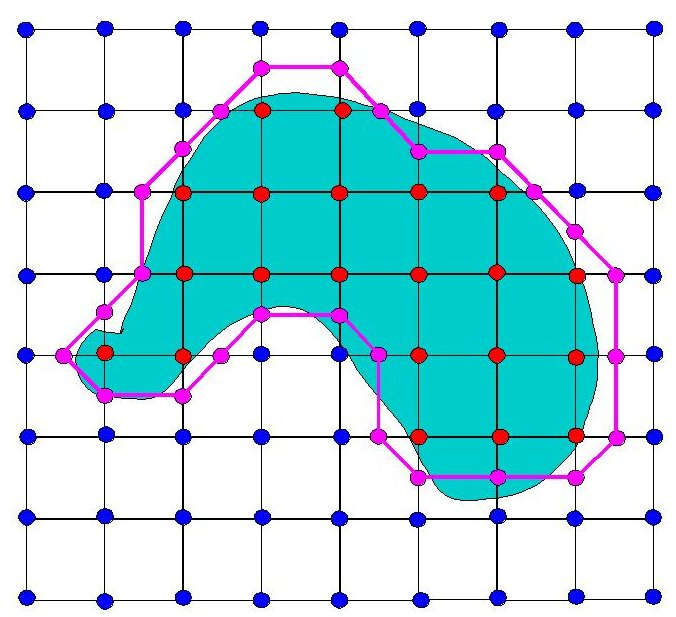
\includegraphics[width=0.8\textwidth]{images/marching_squares.jpg}
    \caption{Using marching squares to extract a shape. From \cite{marching_squares:image}}
    \label{fig:marching_squares}
\end{figure}

The marching cubes algorithm generates as a result a mesh of triangles which can be reduced to the desired resolution by applying some mesh decimation techniques. Once this has been done the volume can be rendered very efficiently using standard rendering techniques.

There are some constraints associated with using surface extraction for volume visualisation. Firstly the number of primitives required to represent certain volumes may be prohibitively high. As an extreme you can imagine trying to extract surfaces from the volumetric representation of a dust cloud; in this case it would not be practical to do so and in other situations an accuracy/efficiency trade off must be found. Also, there is a certain amount of information loss with this technique, importantly the intensity values are lost.

For this project surface extraction could prove useful for generating a rough overview of the scan being worked on that uncertainty data or other information can be overlayed on. If however it is not possible to get a good enough extraction from the data then a reference image, also known as an imposter, could be used instead.

\newpage
\subsection{Uncertainty Visualisation\cite{uncertaintyoverview}}
Uncertainty visualisation tackles the problem of trying to represent the ambiguity or uncertainty in a some data or a model when visualising it.

Most data visualisation techniques implicitly assume that all of the data being used is perfect and because of this create visualisations that are misleading or appear to represent with great precision a model when in fact the underlying data cannot be that sure.

One of the reason that a lot of visualisations leave this kind of information out is that it can be quite to visualise the uncertainty. When creating a visualisation there is an inherent restriction on the dimensions that you can exploit to represent information.

Consider the general problem of creating a visualisation from an n-dimensional dataset and suppose that we are creating a 3D visualisation. In this case we need to somehow map each n-dimensional data point to a ‘dimension’ in our visualisation. The dimensions we can control are space (x, y, z), time and colour (RGB/HSV). The art of data visualisation is to find an intuitive mapping to these and to creatively reuse these dimensions to illustrate different features.

The issue when it comes to uncertainty visualisation is that most of these dimensions have already been used up with the data itself and so finding intuitive representations for uncertainty is difficult.

To get an idea of what is possible with visualisation techniques here are some examples that have been applied successfully in the past.

\begin{figure}[h]
    \centering
	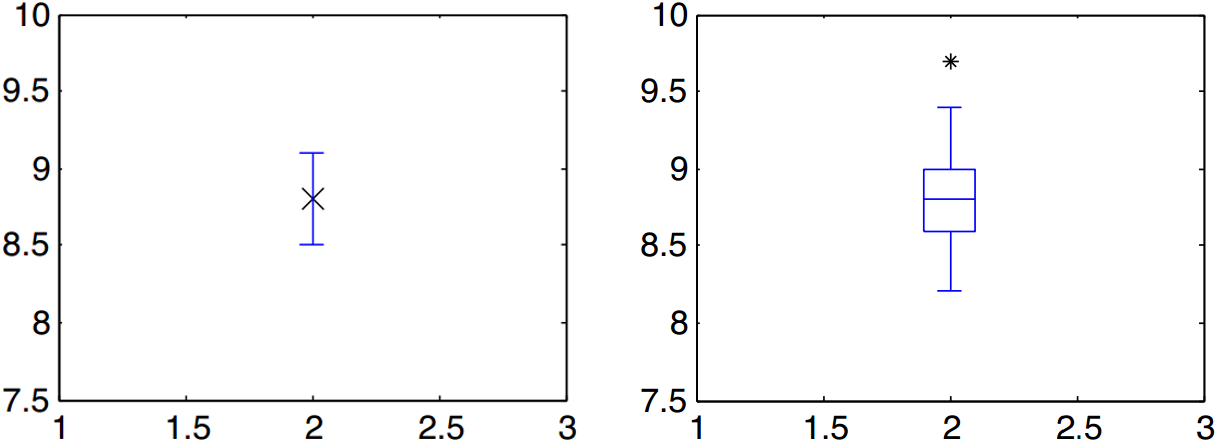
\includegraphics[width=0.8\textwidth]{images/error_bars.png}
    \caption{Left: Error Bar, Right: Box and Whisker Plot. From \cite{uncertaintyoverview}}
    \label{fig:error_bars}
\end{figure}

Error bars are possibly the simplest form of uncertainty visualisation possible and are commonly found on graphs. They make use of one spatial dimension. An extension of this technique is the box and whisker plot which adds some idea of variance and range. An example of both is shown in Figure~\ref{fig:error_bars}.

\begin{figure}[h]
    \centering
	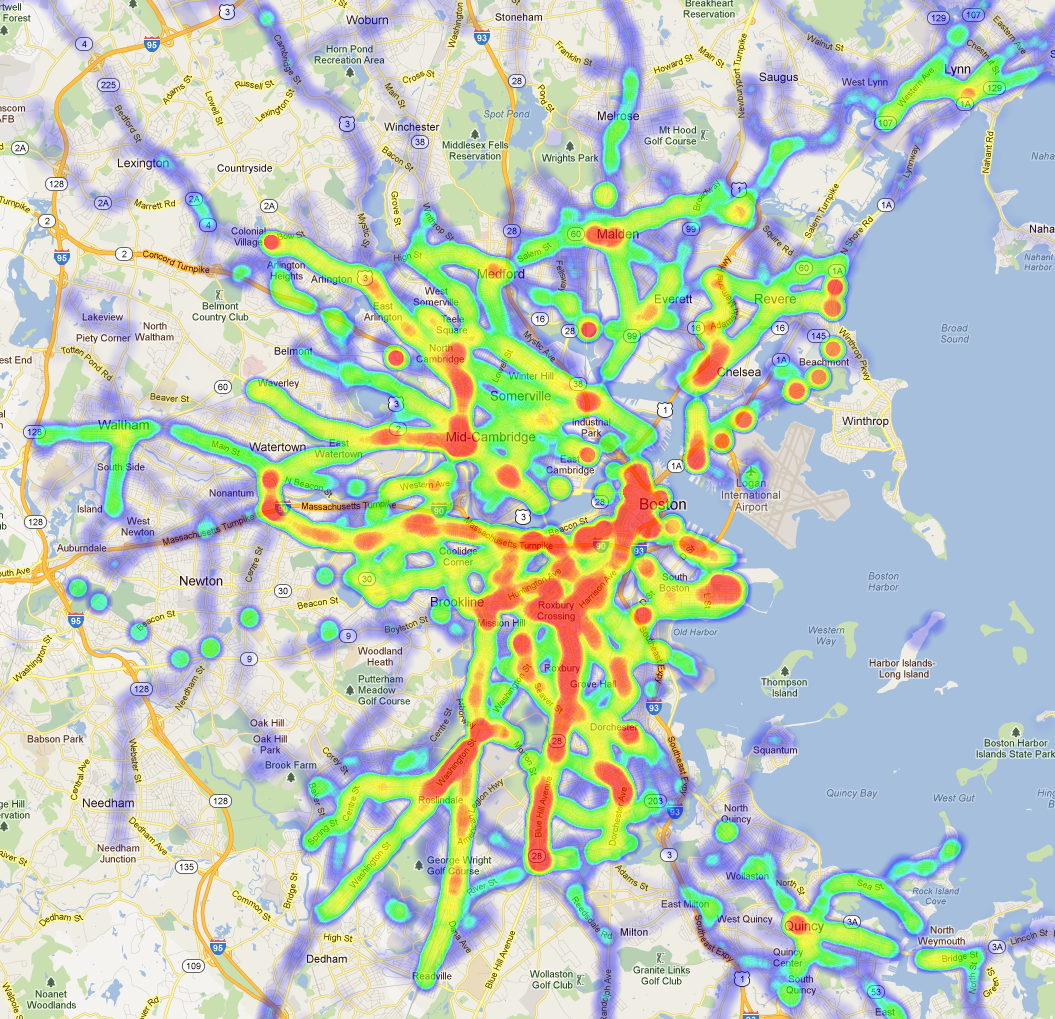
\includegraphics[width=0.8\textwidth]{images/heatmap.png}
    \caption{An example heatmap. From \cite{heatmap}}
    \label{fig:heatmap}
\end{figure}

Colour can be very effective at communicating information. A heatmap uses a range of colours to represent intensity data in a certain range. Transparency can also be used though care must be taken to not over complicate the visualisation. An example of using both colour and transparency is shown in Figure~\ref{fig:heatmap}.

Time is a useful dimension to exploit but is more suited to some visualisations than others. When combined with a different dimension, such as colour, an animation can be produced that can draw the viewers attention.

In particular a team at the Vienna University of Technology have written a paper on attractive flicker which is designed to draw the viewers attention to a particular point in a cluttered scene\cite{attractiveflicker}. Figure~\ref{fig:error_bars} illustrates this idea.

\begin{figure}[h]
    \centering
	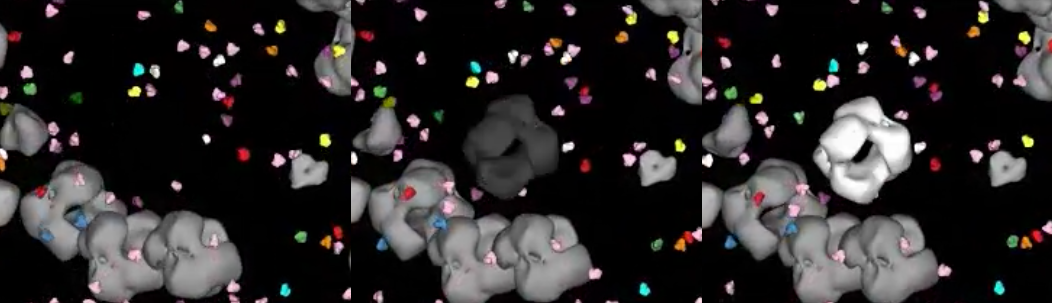
\includegraphics[width=0.8\textwidth]{images/flicker.png}
    \caption{The three frames show a molecule being highlighted as it flickers. From \cite{attractiveflicker}}
    \label{fig:flicker}
\end{figure}

This technique could be useful for illustrating the area of greatest uncertainty or highlighting the scan plane.

When visualising uncertainty in particular you must consider which extreme you would like to draw attention to. A lot of uncertainty visualisations draw larger attention to high uncertainty areas, for example brighter colours on a heatmap or larger error bars, but it may be the case that the viewer is interested in areas of high certainty as this is what they can draw conclusions from.

The uncertainty that we will be dealing with in this project is in fact a vector quantity, composed of three values. 

\begin{enumerate}
	\item (over)sampling - confidence in our sampling resolution
	\item registration - confidence in registration
	\item bias/intensity - confidence in the intensity.
\end{enumerate}

This extra dimensionality will make visualising the uncertainty harder than it would otherwise be. One aspect that is worth investigating is to see whether the three scalar values can be combined to create one representative value or whether they are better visualised individually.

Another aspect of this project will be proposing (and visualising) the next scan plane. This, and potentially other parts of the project, will involve labelling the data in some way. Work on choosing a good labelling system has been done previously and there are a number of different approaches that can be taken\cite{labelling}.

\begin{figure}[h]
    \centering
	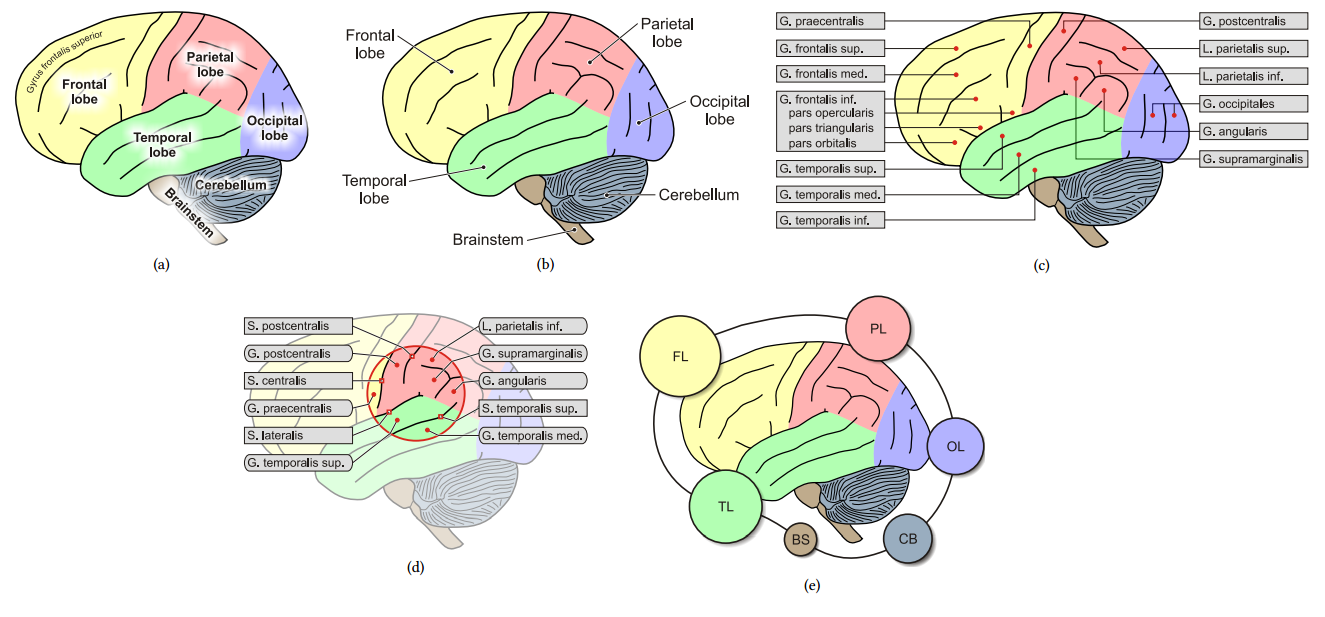
\includegraphics[width=0.8\textwidth]{images/labels.png}
    \caption{A number of different labelling techniques have been studied. Adapted from \cite{labelling}}
    \label{fig:labels}
\end{figure}

If the need for labelling comes up in my project it will be worth investigating these techniques. See Figure~\ref{fig:labels} for examples.
